\documentclass{amsart}
\usepackage[utf8]{inputenc}

\usepackage[parfill]{parskip}
\usepackage[dvipsnames]{xcolor}
\usepackage{microtype}
\usepackage{siunitx}
\DeclareSIUnit\year{yr}
\usepackage{pgfplots}
\usepackage{graphicx}
\usepackage{sidecap}
\sidecaptionvpos{figure}{c}
\usepackage{float}
\usepackage{gensymb}
\usepackage{tkz-euclide}
\usetkzobj{all}
\usepackage{commath}
\usepackage{hyperref}
\usepackage{enumitem}
\usepackage{wasysym}

\renewcommand*{\thefootnote}{\fnsymbol{footnote}}

\newtheorem*{thm}{Theorem}
\newtheorem*{iden}{Identity}
\newtheorem*{lemma}{Lemma}
\theoremstyle{definition}
\newtheorem*{defn}{Definition}
\newtheorem*{ex}{Example}

% russian integral
\usepackage{scalerel}
\DeclareMathOperator*{\rint}{\scalerel*{\rotatebox{17}{$\!\int\!$}}{\int}}

% \qformat{Question \thequestion: \thequestiontitle\hfill}

\begin{document}

\begin{thm}
  If a tangent line has slope $ m $, then the normal line to it has slope $ -1/m $.
\end{thm}

\begin{figure}
  \centering
  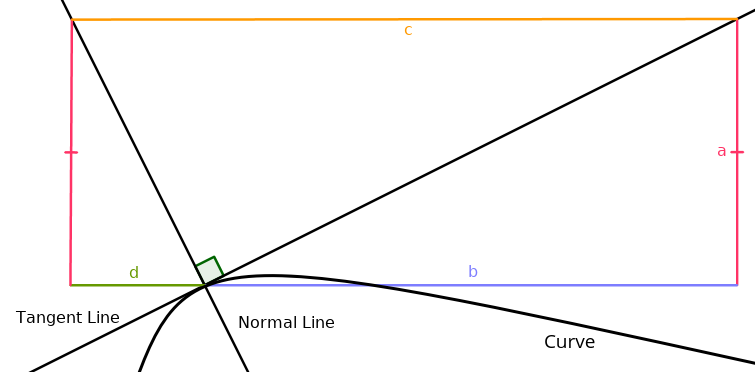
\includegraphics[width=\textwidth]{normal-line-proof}
  \caption{Diagram showing the various triangles used.}
  \label{fig:normal-line-proof}
\end{figure}

\begin{proof}
  Consider the line shown in figure \ref{fig:normal-line-proof}, and let $ m = \frac{a}{b} $ be the slope of the tangent line.
  So the length of the hypotenuse of the $ ab $ triangle is $ \sqrt{a^2 + b^2} $. But $ c = d + b $. Hence the length
  of the hypotenuse of the $ ad $ triangle can be found in two ways:
  \begin{displaymath}
    \sqrt{(d + b)^2 - \left(\sqrt{a^2 + b^2}\right)^2} = \sqrt{a^2 + d^2}.
  \end{displaymath}
  Since all the lengths are positive, we have
  \begin{displaymath}
    d^2 + 2db + b^2 - a^2 - b^2 = a^2 + d^2
  \end{displaymath}
  and therefore
  \begin{displaymath}
    db = a^2 \Rightarrow \frac{d}{a} = \frac{a}{b} = m
  \end{displaymath}
  So the slope of the normal line is simply $ -\frac{a}{d} = -\frac{1}{m} $.
\end{proof}

\end{document}
